% !TEX root = ../chem_ia.tex
\begin{figure}[!htb]
    \centering
    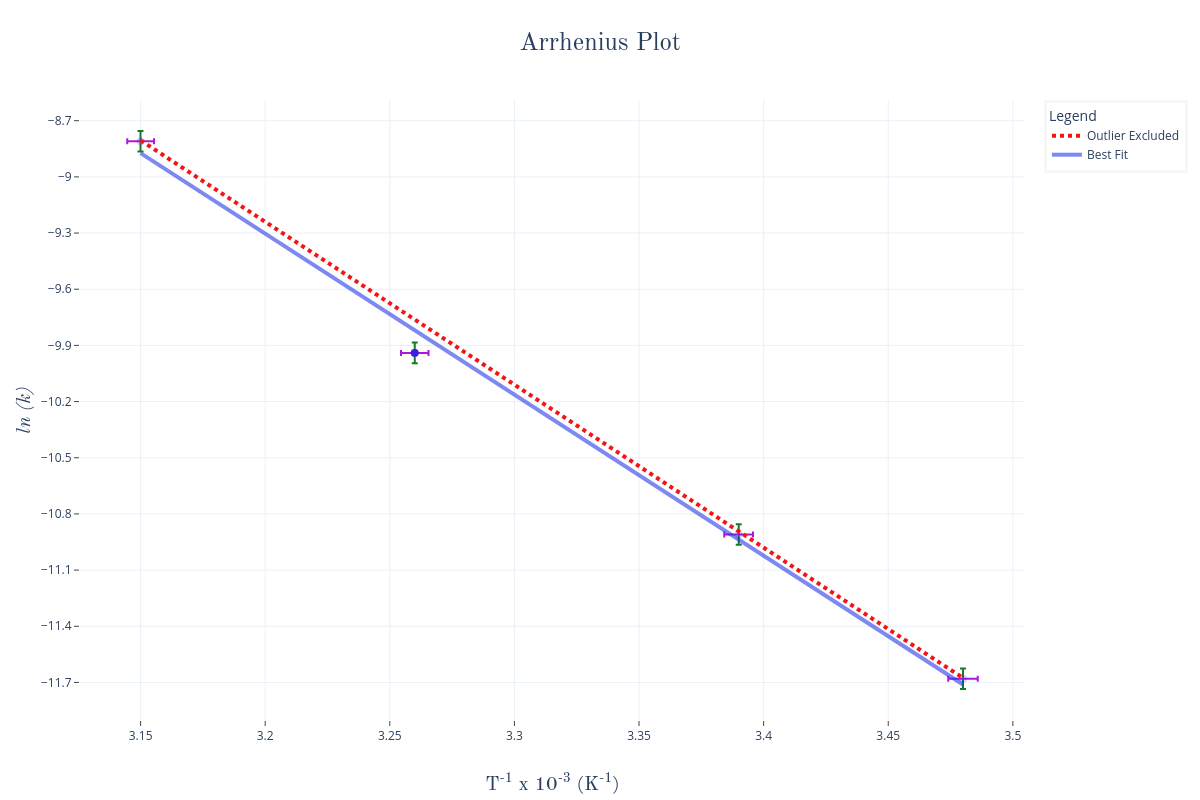
\includegraphics[width=1.0\textwidth]{fig/images/arrhenius.png}
    \caption{Arrhenius plot of $\ln{k}$ versus $\frac{1}{T}$ (scaled by $10^3$), including a best fit line for the general data and an improved trendline with the outlier removed. The blue regression had a final equation of $y = -8.54x + 18.02$, while the red (outlier removed) regression had a final equation of $y = -8.73x + 18.61$.}
    \label{fig:arrhenius}
\end{figure}